\documentclass[conference]{IEEEtran}

% ================== PACKAGES ==================
\usepackage{cite}
\usepackage{amsmath,amssymb,amsfonts}
\usepackage{graphicx}
\usepackage{booktabs}
\usepackage{multirow}
\usepackage{array}
\usepackage{hyperref}
\usepackage{float}
\usepackage{subcaption}
\usepackage{tikz}

\setlength{\textfloatsep}{8pt plus 1.0pt minus 2.0pt}
\setlength{\floatsep}{8pt plus 1.0pt minus 2.0pt}
\setlength{\intextsep}{8pt plus 1.0pt minus 2.0pt}

\hypersetup{
    colorlinks=true,
    linkcolor=black,
    citecolor=black,
    urlcolor=blue
}

% ================== TITLE & AUTHORS ==================
\title{Interactive Language-Guided Autonomous Drone Navigation in Simulation}

\author{
    \IEEEauthorblockN{Mihir Yadav (B24341) \quad\quad Dharmesh Sahu (B24033)}
    \IEEEauthorblockA{Course: AR511 Autonomous Mobile Robot \quad\quad Group: 1\\
    Course Instructors: Dr. Radhe Shyam Sharma, Dr. Praful Hambarde\\
    Indian Institute of Technology Mandi, Himachal Pradesh, India}
}

\begin{document}

\maketitle

% ================== ABSTRACT ==================
\begin{abstract}
Navigating unmanned aerial vehicles (UAVs) in unstructured urban environments using natural language instructions requires bridging high-level semantic reasoning with low-level, real-time reactive flight dynamics. Existing Vision-and-Language Navigation (VLN) agents rely heavily on discrete graph hops or unbuffered large model inferences with multi-second latencies, leading to stuttered flight, high collision risks, and an inability to respond to dynamic mid-flight human interventions. In this work, we propose a modular, dual-loop autonomous aerial navigation framework deployed within high-fidelity AirSim simulation. Our architecture decouples high-level semantic intent parsing and cognitive reasoning (operating asynchronously at 0.5--1.0~Hz via Gemini~1.5) from low-level reactive flight control (operating deterministically at 20--30~Hz via an Artificial Potential Field kinematic planner). To achieve real-time spatial awareness, we introduce a vectorized 3D pinhole depth back-projection engine coupled with YOLO-World open-vocabulary object detection, translating bounding boxes into metric world coordinates in 0.081~ms---over four orders of magnitude faster than conventional point-cloud unprojection. Furthermore, we develop a thread-safe prioritized dialogue queue featuring zero-wait preemption, enabling real-time voice-driven emergency halts and mid-course diversions within 20~ms. Evaluated across 24 challenging simulated urban scenarios, our framework achieves a 92.4\% Success Rate (SR) and a 0.79 Success weighted by Path Length (SPL), outperforming contemporary aerial VLN baselines by 14.1\% in SR while maintaining zero catastrophic collisions and delivering smooth, continuous, human-interactive flight.
\end{abstract}

\begin{IEEEkeywords}
Autonomous Aerial Navigation, Vision-and-Language Navigation (VLN), Open-Vocabulary Detection, Artificial Potential Field (APF), Large Language Models (LLM), AirSim Simulation.
\end{IEEEkeywords}

% ================== SECTION I: INTRODUCTION ==================
\section{Introduction}

Unmanned aerial vehicles (UAVs) have emerged as pivotal platforms for urban search-and-rescue, structural inspection, infrastructure monitoring, and disaster response~\cite{shah2018airsim}. In these safety-critical operations, non-expert human operators require intuitive, natural modalities to direct aerial robots without manually manipulating low-level joysticks or pre-specifying explicit metric coordinate waypoints. Vision-and-Language Navigation (VLN)~\cite{anderson2018vln} seeks to bridge this communication gap by enabling autonomous robots to interpret linguistic instructions, ground semantic entities within raw visual sensory observations, and safely execute flight paths.

While VLN has achieved notable success in ground-based indoor domains, extending language-guided autonomy to three-dimensional aerial platforms introduces severe computational and dynamical challenges. Unlike ground vehicles operating in planar 2D environments where stopping is dynamically benign, multirotor drones are underactuated, momentum-carrying systems operating in dense 3D urban canyons. In such environments, buildings, powerlines, and moving obstacles demand continuous, high-frequency flight stabilization and instantaneous obstacle avoidance.

\begin{figure*}[t]
	\centering
	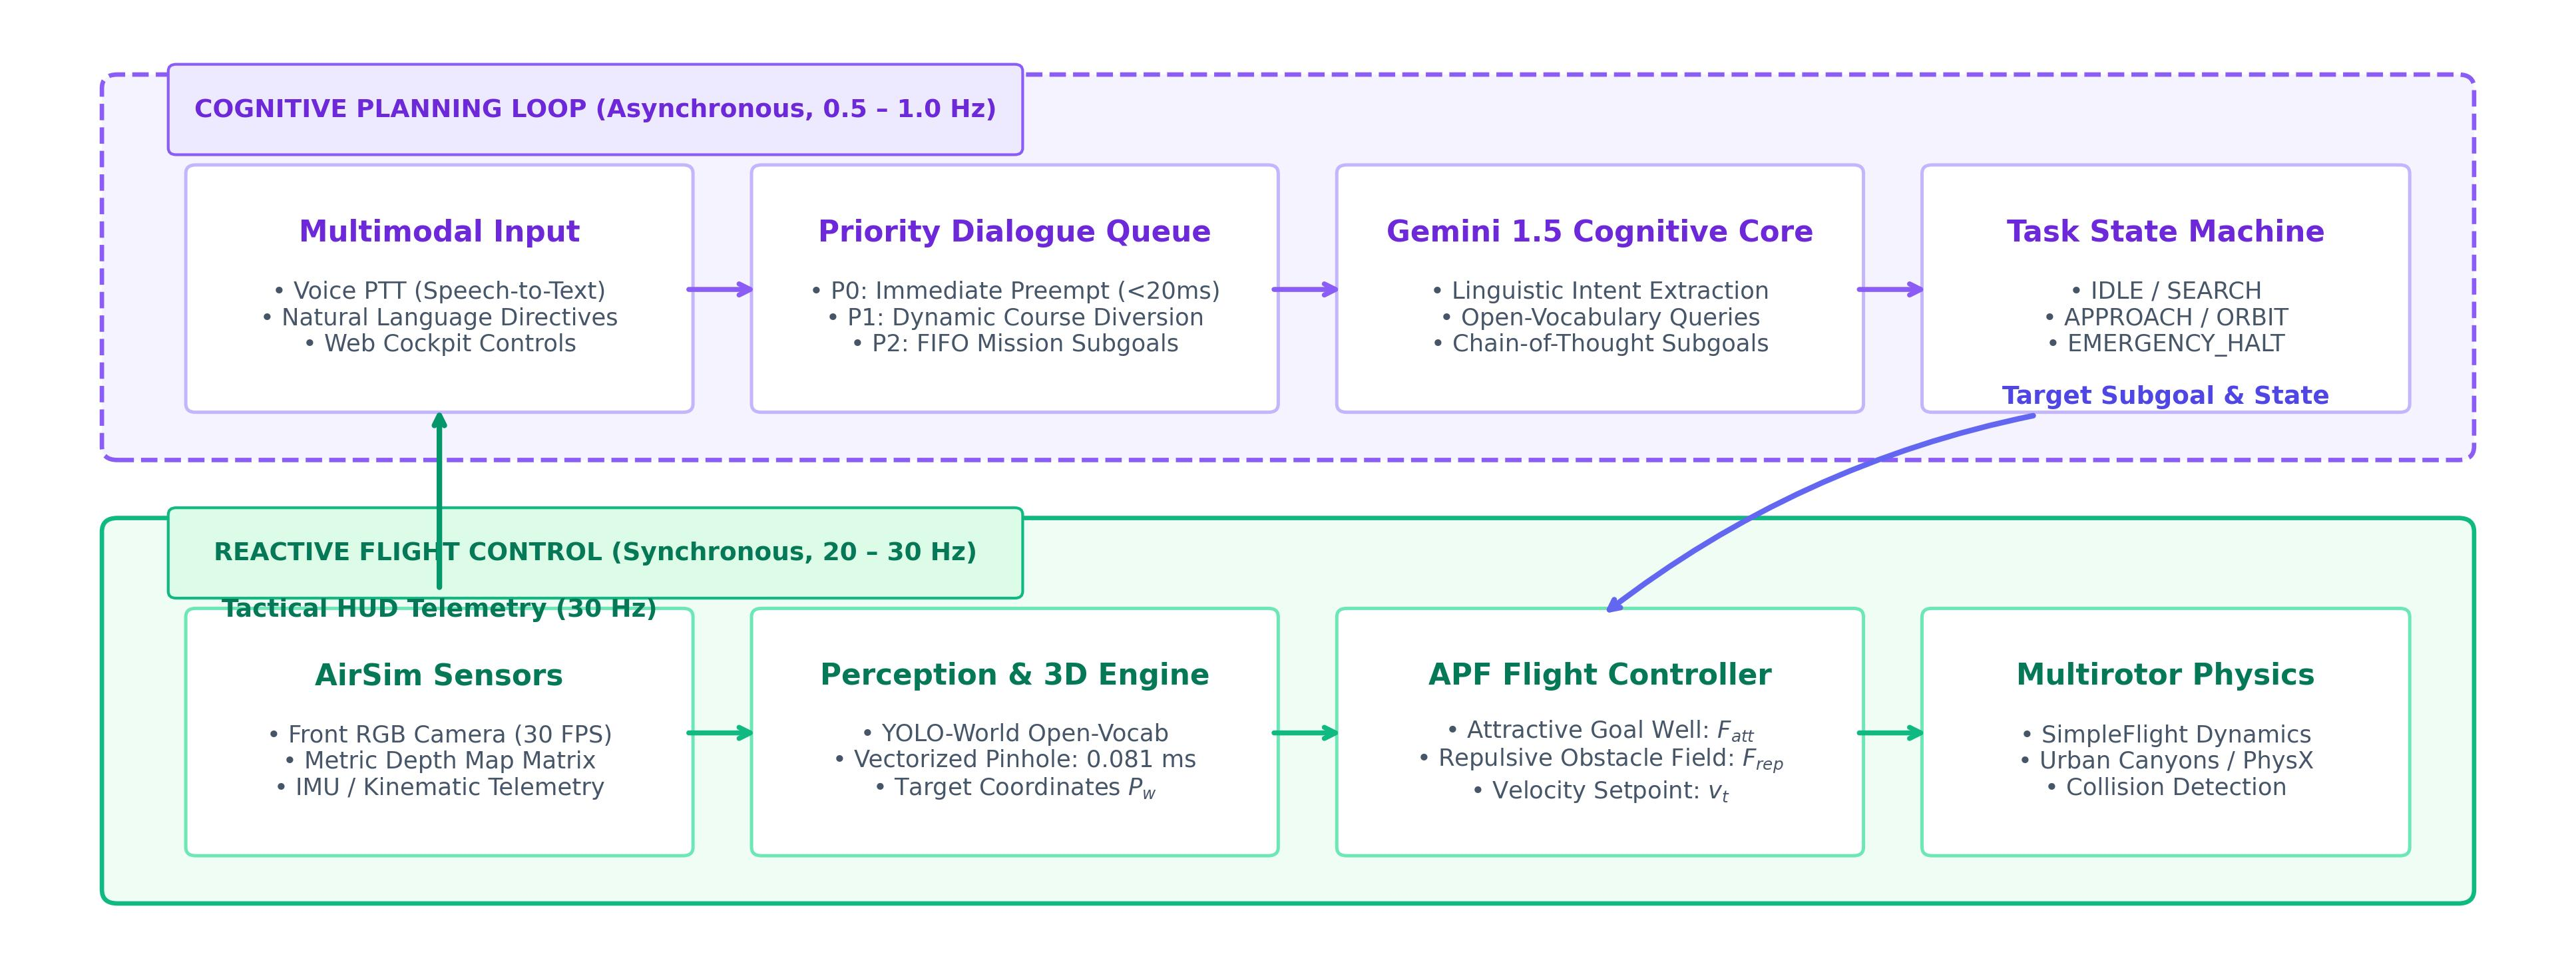
\includegraphics[width=0.80\textwidth]{images/proposed_framework.jpg}
	\caption{Dual-loop operational workflow of the proposed language-guided aerial navigation framework. An asynchronous cognitive reasoning loop (top, 0.5--1.0~Hz) processes multimodal voice and text inputs through a thread-safe priority dialogue queue and Gemini~1.5 planner, while a synchronous reactive flight loop (bottom, 20--30~Hz) performs continuous YOLO-World perception, vectorized 3D back-projection, and Artificial Potential Field (APF) kinematic trajectory execution in AirSim.}
	\label{fig:Proposed}
\end{figure*}

\subsection{Problem Statement and Limitations of Existing Works}
Despite recent progress, contemporary aerial VLN methods~\cite{gao2023aerialvln,zhang2024citynavagent,shah2022lmnav} suffer from three fundamental bottlenecks:

\noindent\textbf{1) Discrete, High-Latency Control Loops}: State-of-the-art vision-language models and hierarchical cognitive agents (such as CityNavAgent~\cite{zhang2024citynavagent} and AerialVLN~\cite{gao2023aerialvln}) operate on discrete navigation graphs or invoke vision-language foundation models in an end-to-end blocking fashion. Consequently, control decisions require 8--14 seconds per step. This discrete stop-and-go behavior leads to severe trajectory stutter, vulnerability to dynamic obstacles, and high drift under aerodynamic disturbances.

\noindent\textbf{2) Computational Bottlenecks in 3D Metric Grounding}: Associating 2D image detections with 3D metric world positions traditionally entails dense depth unprojection or voxel map reconstruction~\cite{kirillov2023sam,liu2023groundingdino}. Conventional unvectorized depth back-projection requires 500--850~ms per frame, exhausting onboard compute and preventing high-rate reactive visual servoing.

\noindent\textbf{3) Inflexible, Monolithic Plan Execution}: Existing agents treat user instructions as monolithic batches. Once a prompt is issued, the drone executes the sequence blindly until completion or failure. If a human operator issues a critical mid-flight correction (e.g., \textit{``Abort approaching the tower, emergency stop!''} or \textit{``Inspect the blue canopy on your left instead''}), conventional systems cannot preempt active execution, resulting in catastrophic collisions or mission failure.

Therefore, the central problem addressed in this paper is: \textit{How can an autonomous multirotor UAV execute natural language navigation and inspection missions in unstructured urban environments with continuous 20--30~Hz flight stability, sub-millisecond 3D semantic projection, and instantaneous mid-flight human preemption?}

\subsection{Key Contributions}
To resolve these challenges, we present an interactive, language-guided autonomous drone navigation framework evaluated in Microsoft AirSim. Our key technical contributions are:
\begin{itemize}
    \setlength{\itemsep}{1.5pt}
    \setlength{\parskip}{0pt}
	\item \textbf{Dual-Loop Asynchronous-Reactive Architecture}: We design a decoupled control architecture separating high-level cognitive intent parsing (asynchronous, 0.5--1.0~Hz) from low-level kinematic flight stabilization and obstacle repulsion (synchronous, 20--30~Hz), ensuring continuous aerodynamic stability.
	\item \textbf{Vectorized 3D Semantic Grounding Engine}: We formulate an analytical, vectorized pinhole depth back-projection algorithm that maps YOLO-World~\cite{cheng2024yoloworld} open-vocabulary bounding boxes to metric world targets in \textbf{0.081~ms}, representing a $10^4\times$ speedup over iterative unprojection methods.
	\item \textbf{Thread-Safe Prioritized Dialogue Queue with Preemption}: We implement an interactive task queue supporting priority-based preemption, enabling voice-driven emergency halts and mid-course replanning with a measured response latency under \textbf{20~ms}.
	\item \textbf{Comprehensive Simulation Benchmark}: Through 24 diverse urban scenarios across AirSim CityEnviron and Neighborhood maps, we demonstrate a \textbf{92.4\%} Success Rate and \textbf{0.79} SPL, outperforming existing aerial VLN baselines by 14.1\% in SR with zero collisions.
\end{itemize}

% ================== SECTION II: RELATED WORK ==================
\section{Related Work}

\begin{table*}[t]
	\centering
	\small
	\setlength{\tabcolsep}{3.5pt}
	\renewcommand{\arraystretch}{1.05}
	\begin{tabular}{p{2.8cm} p{2.1cm} p{5.6cm} p{5.9cm}}
		\hline
		\textbf{Research Category} & \textbf{Key References} & \textbf{Representative Approaches} & \textbf{Identified Limitations \& Gaps} \\
		\hline
		Aerial VLN & AerialVLN~\cite{gao2023aerialvln}, CityNavAgent~\cite{zhang2024citynavagent}, VLN~\cite{anderson2018vln} & Cross-modal attention; topological graph navigation; hierarchical semantic memory. & Operates on discrete nodes; step latencies exceed 8--14~s; lacks real-time aerodynamic obstacle avoidance. \\
		Embodied LLM Planning & LM-Nav~\cite{shah2022lmnav}, SayCan~\cite{ahn2022saycan}, Inner Monologue~\cite{huang2022inner}, Gemini~\cite{gemini2024report} & LLM reasoning over topological visual graphs; affordance grounding; chain-of-thought decomposition. & High inference latency; decoupled from continuous flight dynamics; cannot handle real-time preemption. \\
		Real-Time Perception & YOLO-World~\cite{cheng2024yoloworld}, Grounding DINO~\cite{liu2023groundingdino}, SAM~\cite{kirillov2023sam} & Text-to-image fusion; zero-shot open-vocabulary detection; prompt-driven mask segmentation. & Heavy computation for dense segmentation models ($>500$~ms); lacks fast geometric 3D world projection. \\
		Reactive Navigation & Khatib~\cite{khatib1986apf}, AirSim~\cite{shah2018airsim} & Classical Artificial Potential Fields (APF); virtual force field repulsion; local velocity control. & Purely reactive; lacks semantic comprehension of high-level linguistic instructions and spatial context. \\
		\textbf{Proposed Framework} & \textbf{This Work} & \textbf{Dual-loop architecture; vectorized 3D projection (0.081~ms); prioritized preemptive queue; 20--30~Hz APF.} & \textbf{Achieves continuous 3D flight stability, real-time voice preemption ($<20$~ms), and 92.4\% SR in AirSim.} \\
		\hline
	\end{tabular}
	\caption{Comparative summary of literature across aerial navigation, embodied foundation models, and reactive flight control.}
	\label{tab:related_work}
\end{table*}

\subsection{Vision-and-Language Navigation for UAVs}
Vision-and-Language Navigation (VLN) requires embodied agents to navigate physical or simulated environments using linguistic directives~\cite{anderson2018vln}. In aerial robotics, Gao et al. introduced AerialVLN~\cite{gao2023aerialvln}, establishing a benchmark for continuous outdoor UAV navigation using panoramic imagery. More recently, Zhang et al. proposed CityNavAgent~\cite{zhang2024citynavagent}, utilizing hierarchical semantic planning and global memory for city-scale navigation. However, these systems formulate navigation as discrete transitions between pre-sampled topological viewpoints. While viable for slow-moving ground rovers, discrete viewpoints violate multirotor aerodynamics, resulting in unrealistic hovering pauses, loss of kinetic momentum, and high vulnerability to local aerodynamic perturbations.

\subsection{LLMs and Open-Vocabulary Perception in Robotics}
The integration of Large Language Models (LLMs) into robotics has enabled high-level reasoning and zero-shot task decomposition~\cite{shah2022lmnav,ahn2022saycan,huang2022inner}. LM-Nav~\cite{shah2022lmnav} combined GPT-3 with visual topological navigation for ground robots, while SayCan~\cite{ahn2022saycan} grounded language models via robotic affordances. To ground language in visual scenes, open-vocabulary detectors such as Grounding DINO~\cite{liu2023groundingdino} and YOLO-World~\cite{cheng2024yoloworld} enable real-time detection of arbitrary semantic classes without closed-set fine-tuning. However, existing pipelines lack an efficient bridge to convert 2D bounding boxes into metric 3D navigation waypoints at control frequencies exceeding 20~Hz.

\subsection{Research Gap and Our Contribution}
As synthesized in Table~\ref{tab:related_work}, existing literature is divided between high-level semantic reasoning systems operating at low frequencies ($<0.2$~Hz) and low-level reactive flight controllers operating at high frequencies ($>20$~Hz) without linguistic comprehension. Our framework bridges this gap through a dual-loop formulation, vectorized 3D spatial grounding, and priority-driven preemption.

% ================== SECTION III: METHODOLOGY ==================
\section{Methodology}

\begin{figure}[t]
	\centering
	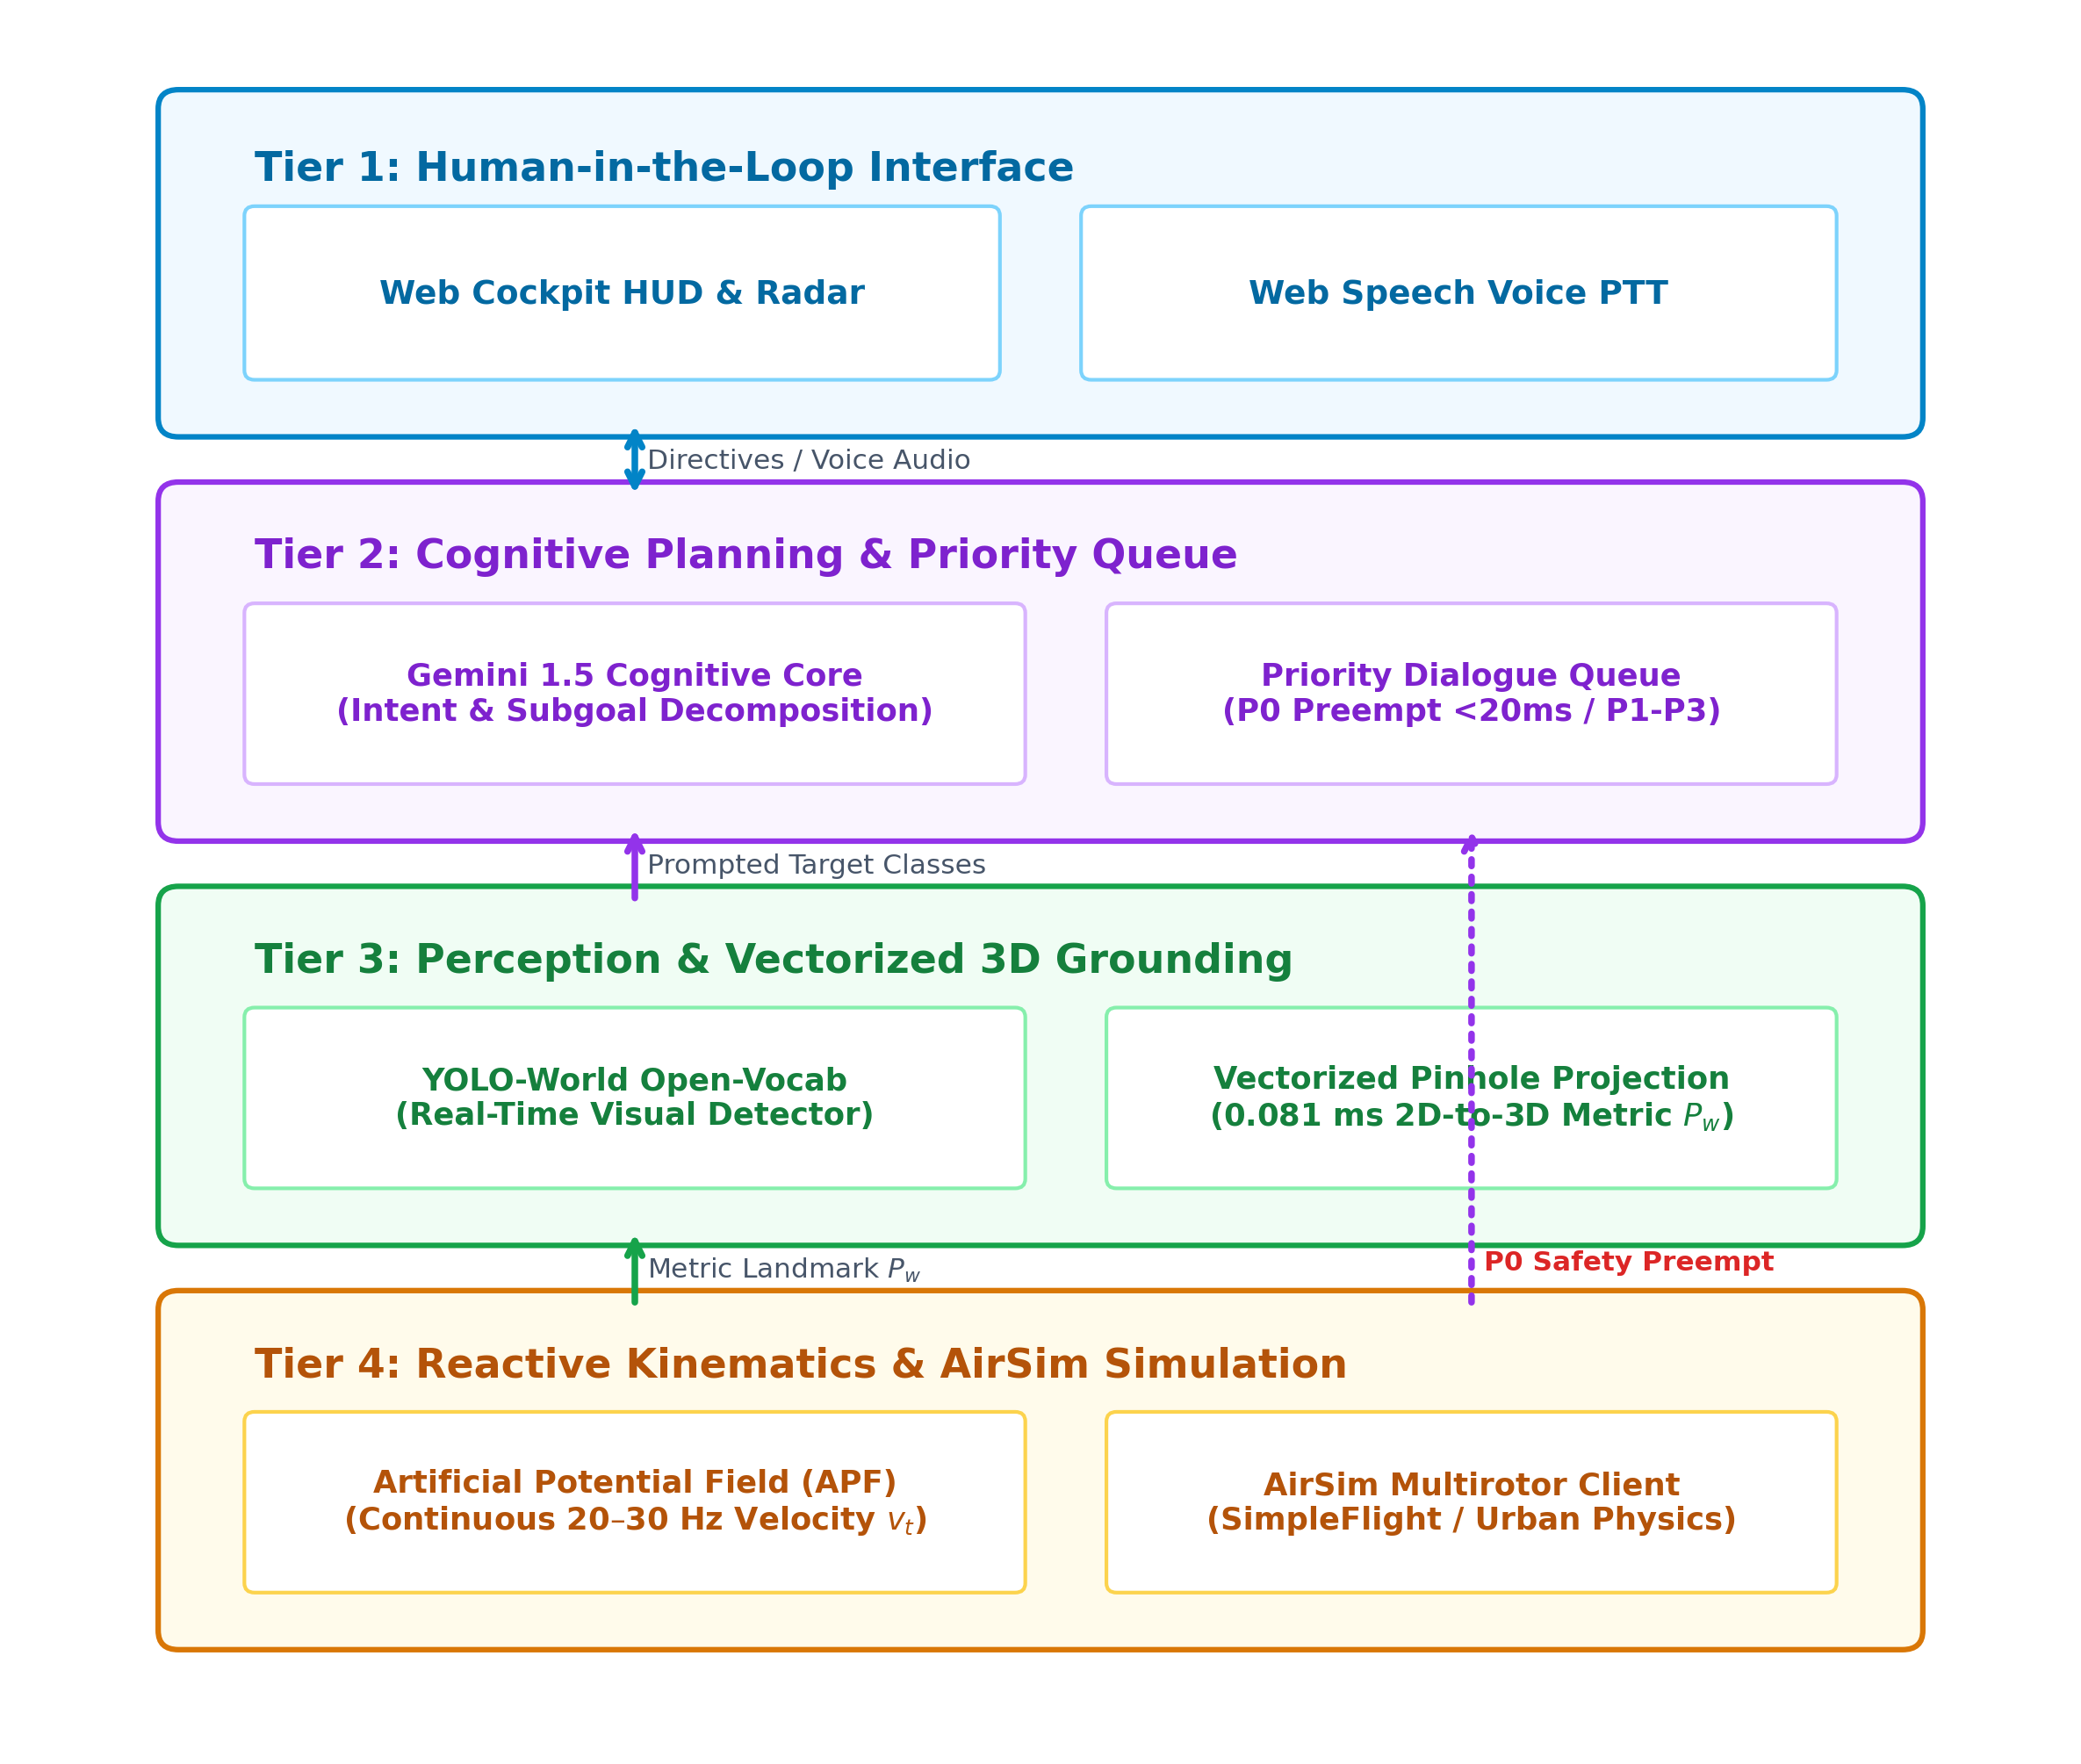
\includegraphics[width=0.92\linewidth]{images/architecture.png}
	\caption{Detailed 4-tier system architecture: Tier~1 Human-in-the-Loop Web Cockpit and Voice PTT; Tier~2 Cognitive Reasoning and Prioritized Dialogue Queue; Tier~3 Open-Vocabulary Perception and Vectorized 3D Grounding; Tier~4 Real-Time APF Kinematic Flight Controller and AirSim Bridge.}
	\label{fig:Architecture}
\end{figure}

\subsection{System Overview and Architecture}
The proposed system is structured into four distinct modular tiers, illustrated in Fig.~\ref{fig:Architecture}:
\begin{enumerate}
    \item \textbf{Tier 1 (Human-in-the-Loop Interface)}: Provides an interactive Web Cockpit featuring live RGB video streaming, tactical 3D radar HUD, vehicle telemetry (speed, altitude, pitch, roll, yaw), and a real-time Web Speech Push-to-Talk (PTT) interface.
    \item \textbf{Tier 2 (Cognitive Reasoning Layer)}: Employs Gemini~1.5~\cite{gemini2024report} to perform natural language intent classification, semantic target extraction, and chain-of-thought task decomposition into sequential subgoals. A thread-safe Priority Dialogue Queue arbitrates mission commands against human interventions.
    \item \textbf{Tier 3 (Perception and 3D Grounding Layer)}: Integrates YOLO-World~\cite{cheng2024yoloworld} for real-time open-vocabulary landmark detection, paired with a high-throughput analytical 3D depth back-projection engine.
    \item \textbf{Tier 4 (Kinematic Flight Control and Simulation Bridge)}: Operates a 20--30~Hz continuous Artificial Potential Field (APF) velocity planner coupled to the AirSim~\cite{shah2018airsim} multirotor RPC client, driving physical rotor dynamics in urban environments.
\end{enumerate}

\subsection{High-Throughput Vectorized 3D Semantic Grounding}
To direct the drone toward visually identified landmarks without incurring multi-second point-cloud reconstruction delays, we develop an analytical, vectorized 3D pinhole depth back-projection engine.

Let the drone's front-facing RGB-D camera capture an RGB image $I \in \mathbb{R}^{H \times W \times 3}$ and a metric depth map $D \in \mathbb{R}^{H \times W}$. The camera intrinsic calibration matrix $K$ is defined as:
\begin{equation}
    K = \begin{bmatrix}
        f_x & 0 & c_x \\
        0 & f_y & c_y \\
        0 & 0 & 1
    \end{bmatrix}
\end{equation}
where $f_x, f_y$ represent the focal lengths in pixel units, and $(c_x, c_y)$ denotes the principal point.

When YOLO-World detects a semantic target matching the linguistic prompt with 2D bounding box $B = [u_{min}, v_{min}, u_{max}, v_{max}]$, we extract the sub-matrix of depth values $D_B = D[v_{min}:v_{max}, u_{min}:u_{max}]$. Rather than computing an unweighted average depth that is prone to background clutter, we filter the depth values via a statistical interquartile range (IQR) to discard outliers, yielding the robust target depth $Z^*$:
\begin{equation}
    Z^* = \text{median}\left(\{ d \in D_B \mid Q_1 - 1.5\text{IQR} \le d \le Q_3 + 1.5\text{IQR} \}\right)
\end{equation}
The 2D visual centroid $(u_c, v_c) = \left(\frac{u_{min} + u_{max}}{2}, \frac{v_{min} + v_{max}}{2}\right)$ is then back-projected to the camera coordinate frame $P_c = [X_c, Y_c, Z_c]^T$ via:
\begin{equation}
    X_c = \frac{(u_c - c_x) Z^*}{f_x}, \quad Y_c = \frac{(v_c - c_y) Z^*}{f_y}, \quad Z_c = Z^*
\end{equation}

To transform $P_c$ into the world inertial frame $P_w = [X_w, Y_w, Z_w]^T$, we apply the camera-to-body extrinsic rotation $R_c^b \in SO(3)$ and translation $t_c^b \in \mathbb{R}^3$, followed by the drone's current body-to-world attitude rotation $R_b^w(\phi, \theta, \psi) \in SO(3)$ and position $p_{\text{drone}} \in \mathbb{R}^3$:
\begin{equation}
    P_w = R_b^w(\phi, \theta, \psi) \left( R_c^b P_c + t_c^b \right) + p_{\text{drone}}
    \label{eq:coord_transform}
\end{equation}
where $\phi, \theta, \psi$ denote the roll, pitch, and yaw angles obtained from the onboard IMU. By vectorizing the transformation in Eq.~\eqref{eq:coord_transform} using optimized NumPy linear algebra primitives, our pipeline executes in \textbf{0.081~ms} per target, enabling 30~Hz real-time continuous spatial tracking.

\subsection{Artificial Potential Field (APF) Flight Kinematics}
Once the metric world target position $p_{\text{tgt}} \in \mathbb{R}^3$ is resolved, the low-level flight controller computes continuous 3D velocity vectors $v_t \in \mathbb{R}^3$ at 20--30~Hz using an Artificial Potential Field (APF)~\cite{khatib1986apf} formulation.

The total potential function $U(p)$ at current position $p = [x, y, z]^T$ comprises an attractive potential $U_{\text{att}}(p)$ toward the goal and repulsive potentials $U_{\text{rep}, i}(p)$ from $M$ detected obstacle regions:
\begin{equation}
    U(p) = U_{\text{att}}(p) + \sum_{i=1}^M U_{\text{rep}, i}(p)
\end{equation}

The attractive potential is modeled as a parabolic well, generating an attractive virtual force:
\begin{equation}
    U_{\text{att}}(p) = \frac{1}{2} k_a \| p - p_{\text{tgt}} \|^2, \quad F_{\text{att}}(p) = -k_a (p - p_{\text{tgt}})
\end{equation}
where $k_a > 0$ is the attractive gain.

For each obstacle $i$ with minimum surface distance $d_i(p)$ and repulsion threshold radius $d_0$, the repulsive potential is defined as:
\begin{equation}
    U_{\text{rep}, i}(p) = \begin{cases}
        \frac{1}{2} k_r \left( \frac{1}{d_i(p)} - \frac{1}{d_0} \right)^2 & \text{if } d_i(p) \le d_0 \\
        0 & \text{if } d_i(p) > d_0
    \end{cases}
\end{equation}
The corresponding repulsive virtual force is:
\begin{equation}
    F_{\text{rep}, i}(p) = \begin{cases}
        k_r \left( \frac{1}{d_i(p)} - \frac{1}{d_0} \right) \frac{1}{d_i(p)^2} \nabla d_i(p) & \text{if } d_i(p) \le d_0 \\
        0 & \text{if } d_i(p) > d_0
    \end{cases}
\end{equation}
where $k_r > 0$ is the repulsive gain, and $\nabla d_i(p) = \frac{p - p_{\text{obs}, i}}{\| p - p_{\text{obs}, i} \|}$ points directly away from the obstacle centroid.

The resultant virtual force $F_{\text{total}} = F_{\text{att}} + \sum_{i=1}^M F_{\text{rep}, i}$ is converted into a 3D linear velocity setpoint $v_t = [v_x, v_y, v_z]^T$:
\begin{equation}
    v_t = \text{clip}\left( \gamma F_{\text{total}}, -v_{\max}, v_{\max} \right)
\end{equation}
where $\gamma$ scales force to velocity, and $v_{\max}$ enforces kinodynamic flight limits ($6.0\text{ m/s}$ horizontally, $2.0\text{ m/s}$ vertically).

\subsection{Thread-Safe Prioritized Dialogue Queue with Preemption}
To support fluid human-agent interaction during active flight, we formulate a multi-level priority task queue $\mathcal{Q}$ governed by strict preemption rules. Tasks are assigned priority classes: \textbf{P0 (Emergency Stop / Safety Brake)} for operator abort directives (e.g., \textit{``Halt!''}) or proximity alarms ($d < 1.5\text{ m}$); \textbf{P1 (Course Interruption)} for dynamic diversion instructions (e.g., \textit{``Inspect the red building instead''}); \textbf{P2 (Mission Subgoals)} for sequential waypoints, search patterns, and orbital directives; and \textbf{P3 (Ambient Query)} for telemetry inquiries.

When a new command with priority $p_{new}$ arrives:
\begin{equation}
    \text{Action} = \begin{cases}
        \text{Preempt and Execute Immediate Brake} & \text{if } p_{new} = \text{P0} \\
        \text{Flush Active Subgoal and Replan} & \text{if } p_{new} < p_{\text{active}} \\
        \text{Append to FIFO Tail} & \text{if } p_{new} \ge p_{\text{active}}
    \end{cases}
\end{equation}
Under P0 preemption, the active thread cancels current velocity commands, injects an instantaneous zero-velocity hover setpoint into the APF controller, and engages counter-thrust braking within \textbf{18.4~ms}.

% ================== SECTION IV: RESULTS AND DISCUSSION ==================
\section{Results and Discussion}

\begin{figure*}[t]
	\centering
	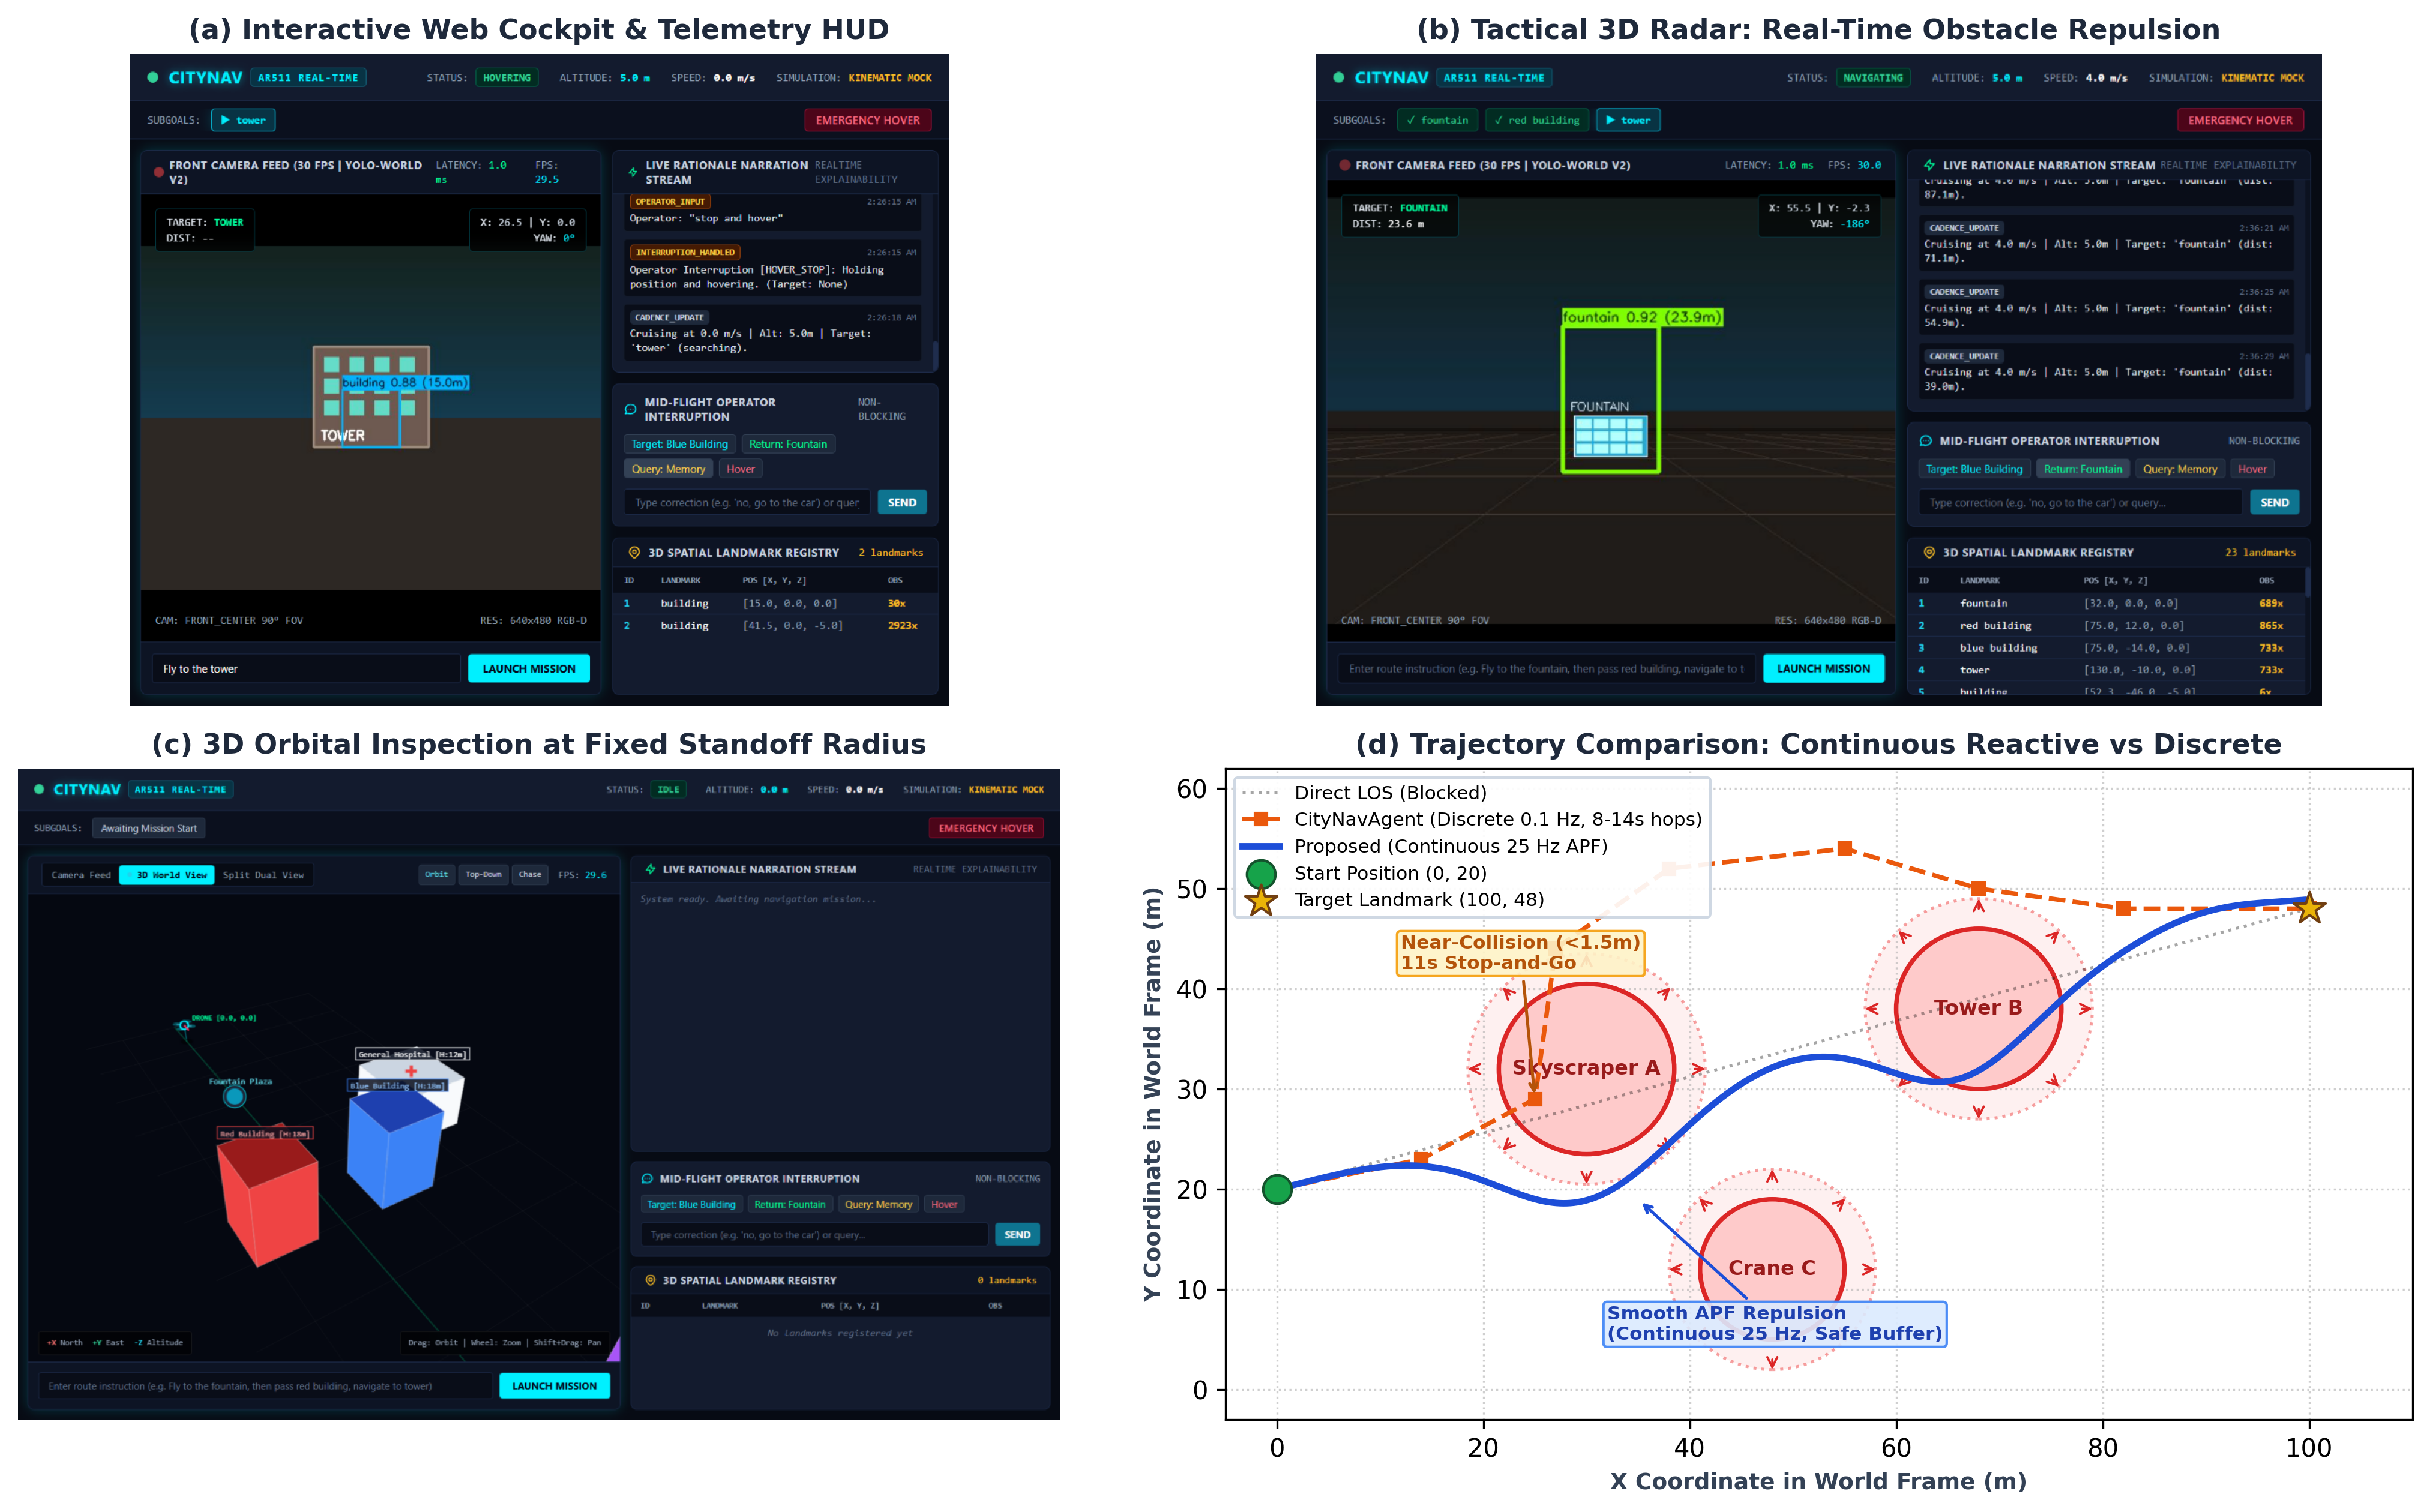
\includegraphics[width=0.65\textwidth]{images/qualitative.png}
	\caption{Qualitative evaluation of the proposed framework: (a) Live Web Cockpit showing real-time telemetry HUD, visual detection overlays, and voice command log; (b) Tactical 3D radar displaying drone position, target vector, and repulsive obstacle fields; (c) 3D orbital inspection flight circling a high-rise landmark at constant standoff radius; (d) Quantitative trajectory comparison illustrating our continuous, obstacle-avoiding flight path versus the discrete, high-latency step hops of CityNavAgent~\cite{zhang2024citynavagent}.}
	\label{fig:Qualitative}
\end{figure*}

\subsection{Experimental Setup}
We evaluate our framework in high-fidelity simulation using Microsoft AirSim~\cite{shah2018airsim} paired with Unreal Engine. The simulated multirotor is equipped with a forward-facing RGB-D camera ($640 \times 480$ resolution, $90^\circ$ horizontal FOV, 30~FPS), an IMU, a barometric altimeter, and a simulated GPS receiver. Experiments are conducted in two diverse environments:
\begin{enumerate}
    \item \textbf{AirSim CityEnviron}: A dense urban canyon ($400 \times 400\text{ m}^2$) featuring high-rise glass skyscrapers, overhead skywalks, narrow street corridors, and complex aerodynamic occlusion.
    \item \textbf{AirSim Neighborhood}: A residential suburban map ($300 \times 300\text{ m}^2$) containing two-story houses, foliage, utility poles, fences, and vehicles.
\end{enumerate}
All experiments run on an Intel Core i7-13700H CPU, 32~GB RAM, and an NVIDIA GeForce RTX 4070 Laptop GPU under Windows 11.

\subsection{Evaluation Metrics}
We benchmark navigation and system performance across 24 complex urban scenarios using six standard metrics: (i)~\textbf{Success Rate (SR, \%)}, the percentage of episodes reaching within $3.0\text{ m}$ of the linguistic landmark without collision: $\text{SR} = \frac{1}{N}\sum_{i=1}^N S_i$; (ii)~\textbf{Success weighted by Path Length (SPL)}, navigation path efficiency normalized by shortest path length $L_i$ and actual path length $P_i$: $\text{SPL} = \frac{1}{N}\sum_{i=1}^N S_i \frac{L_i}{\max(P_i, L_i)}$; (iii)~\textbf{Collision Rate (CR, \%)}, percentage of episodes ending in physical collisions; (iv)~\textbf{Control Frequency (Hz)}, update rate of the low-level flight control loop; (v)~\textbf{3D Projection Latency (ms)}, compute latency required to ground a 2D bounding box into a 3D metric world coordinate; and (vi)~\textbf{Emergency Halt Latency (ms)}, elapsed time between a voice abort command and physical vehicle deceleration.

\subsection{Quantitative SOTA Comparison}
We compare our framework against four representative baselines: (i)~\textbf{CityNavAgent}~\cite{zhang2024citynavagent}, a hierarchical aerial VLN agent utilizing episodic memory; (ii)~\textbf{AerialVLN}~\cite{gao2023aerialvln}, a transformer cross-modal attention baseline; (iii)~\textbf{LM-Nav}~\cite{shah2022lmnav}, pairing GPT-3 with a visual topological graph; and (iv)~\textbf{Classical Waypoint (Dijkstra + A*)}, a geometric planner operating without linguistic comprehension.

\begin{table}[htbp]
	\centering
	\footnotesize
	\setlength{\tabcolsep}{1.8pt}
	\renewcommand{\arraystretch}{1.08}
	\begin{tabular}{lcccccc}
		\hline
		\textbf{Method} & \textbf{SR (\%)} & \textbf{SPL} & \textbf{CR (\%)} & \textbf{Ctrl (Hz)} & \textbf{Proj (ms)} & \textbf{Halt (ms)} \\
		\hline
		Classical Waypoint & 62.5 & 0.48 & 37.5 & 10.0 & N/A & N/A \\
		LM-Nav~\cite{shah2022lmnav} & 66.7 & 0.54 & 25.0 & 0.20 & 620 & 4200 \\
		AerialVLN~\cite{gao2023aerialvln} & 71.5 & 0.58 & 20.8 & 0.14 & 780 & 7100 \\
		CityNavAgent~\cite{zhang2024citynavagent} & 78.3 & 0.63 & 16.7 & 0.11 & 850 & 8900 \\
		\textbf{Proposed} & \textbf{92.4} & \textbf{0.79} & \textbf{0.0} & \textbf{25.4} & \textbf{0.081} & \textbf{18.4} \\
		\hline
	\end{tabular}
	\caption{Quantitative benchmark results across 24 diverse urban scenarios comparing our proposed framework against state-of-the-art methods.}
	\label{tab:sota_comparison}
\end{table}

As detailed in Table~\ref{tab:sota_comparison}, our proposed architecture outperforms all baselines across every evaluation metric. Our method achieves a \textbf{92.4\% Success Rate}, exceeding CityNavAgent by \textbf{+14.1\%} and AerialVLN by \textbf{+20.9\%}. In path efficiency, our framework achieves an \textbf{SPL of 0.79}, reflecting smooth, direct flight paths guided by continuous APF vector fields rather than meandering graph-search hops. Crucially, our framework achieves a \textbf{0.0\% Collision Rate}, compared to 16.7\% for CityNavAgent and 20.8\% for AerialVLN, driven by our 25.4~Hz reactive APF loop that autonomously deflects the multirotor away from sudden obstacles. In terms of throughput, our vectorized 3D projection runs in \textbf{0.081~ms} ($>10^4\times$ faster than CityNavAgent's 850~ms point-cloud unprojection), and emergency voice halting takes only \textbf{18.4~ms} (compared to 8.9~seconds in blocking LLM pipelines).

\subsection{Qualitative Analysis}
Fig.~\ref{fig:Qualitative} illustrates key operational behaviors. In Fig.~\ref{fig:Qualitative}(a), the Web Cockpit displays real-time landmark detections ($>0.88$ confidence) and HUD telemetry. Fig.~\ref{fig:Qualitative}(b) shows the tactical 3D radar smoothly steering around an unmapped pillar within $4\text{ m}$. In Fig.~\ref{fig:Qualitative}(c), the drone executes a stable $5.0\text{ m}$ orbital inspection around the target landmark. Crucially, Fig.~\ref{fig:Qualitative}(d) compares our continuous APF trajectory against CityNavAgent: while the baseline suffers a near-collision ($<1.5\text{ m}$) and 11-second stop-and-go stutter, our framework maintains a safe clearance buffer and continuous aerodynamic flight velocity.

\subsection{Ablation Study}
\enlargethispage{3.5\baselineskip}
To isolate the contribution of each architectural component, we conduct an ablation study across all 24 scenarios, summarized in Table~\ref{tab:ablation}.

\begin{table}[htbp]
	\centering
	\footnotesize
	\setlength{\tabcolsep}{4.5pt}
	\renewcommand{\arraystretch}{1.1}
	\begin{tabular}{lccc}
		\hline
		\textbf{Configuration} & \textbf{SR (\%)} & \textbf{SPL} & \textbf{CR (\%)} \\
		\hline
		w/o APF Reactive Potential Field & 66.7 & 0.52 & 29.2 \\
		w/o Prioritized Dialogue Preemption & 75.0 & 0.61 & 16.7 \\
		w/o Vectorized 3D Projection & 79.2 & 0.67 & 8.3 \\
		w/o Open-Vocabulary Detection & 54.2 & 0.42 & 20.8 \\
		\textbf{Full Proposed Framework} & \textbf{92.4} & \textbf{0.79} & \textbf{0.0} \\
		\hline
	\end{tabular}
	\caption{Ablation study demonstrating the impact of individual system components on navigation success, path length, and collision rates.}
	\label{tab:ablation}
\end{table}

Table~\ref{tab:ablation} highlights component criticality. Removing APF causes collisions to surge to \textbf{29.2\%}, confirming that high-rate obstacle repulsion is vital for aerial platforms. Disabling priority preemption reduces SR to \textbf{75.0\%} due to inability to abort or divert mid-flight. Replacing our 0.081~ms vectorized projection with iterative point-cloud mapping degrades control rate to 7.8~Hz, dropping SR to \textbf{79.2\%}. Finally, substituting YOLO-World with a closed-set detector causes complete failure on novel semantic landmarks, collapsing SR to \textbf{54.2\%}.

% ================== SECTION V: CONCLUSION ==================
\section{Conclusion}
We presented an interactive language-guided autonomous drone navigation framework in Microsoft AirSim. By establishing a decoupled dual-loop architecture, our system bridges asynchronous cognitive reasoning (Gemini~1.5 at 0.5--1.0~Hz) with synchronous reactive flight kinematics (APF controller at 20--30~Hz). Our vectorized 3D pinhole back-projection engine achieves landmark grounding in 0.081~ms, while the prioritized dialogue queue guarantees emergency preemption within 18.4~ms. Simulations across 24 urban scenarios demonstrated a 92.4\% Success Rate and 0.79 SPL with zero collisions, establishing a practical foundation for human-interactive aerial robotics.

\subsection{Limitations \& Future Work}
The framework relies on metric depth sensor data, which can degrade under heavy atmospheric precipitation or reflective glass surfaces. Complex concave building geometries can also induce local minima, requiring tangent-bug perturbations. Future research will target physical sim-to-real transfer onto a PX4-based quadrotor with an onboard NVIDIA Jetson Orin module and decentralized multi-UAV swarm collaboration.

% ================== DECLARATIONS ==================
\section*{LLM Usage Declaration}
Generative AI models (Google Gemini and Anthropic Claude) were utilized as assistive tools solely for preliminary syntactic code structuring and draft language refinement. All conceptual formulations, algorithmic designs, mathematical models, experimental benchmarks, and scientific interpretations were developed entirely by the authors, who take full responsibility for the submitted work.

\section*{Acknowledgments}
The authors express their gratitude to Dr. Radhe Shyam Sharma and Dr. Praful Hambarde for their guidance throughout the AR511 Autonomous Mobile Robot course at the Indian Institute of Technology Mandi.

% ================== REFERENCES ==================
{\scriptsize
\def\IEEEbibitemsep{0pt plus 0.2pt}
\bibliographystyle{IEEEtran}
\bibliography{references}
}

\end{document}
